\documentclass{standalone}
\usepackage{pgfplots}
\pgfplotsset{compat=newest}

\begin{document}
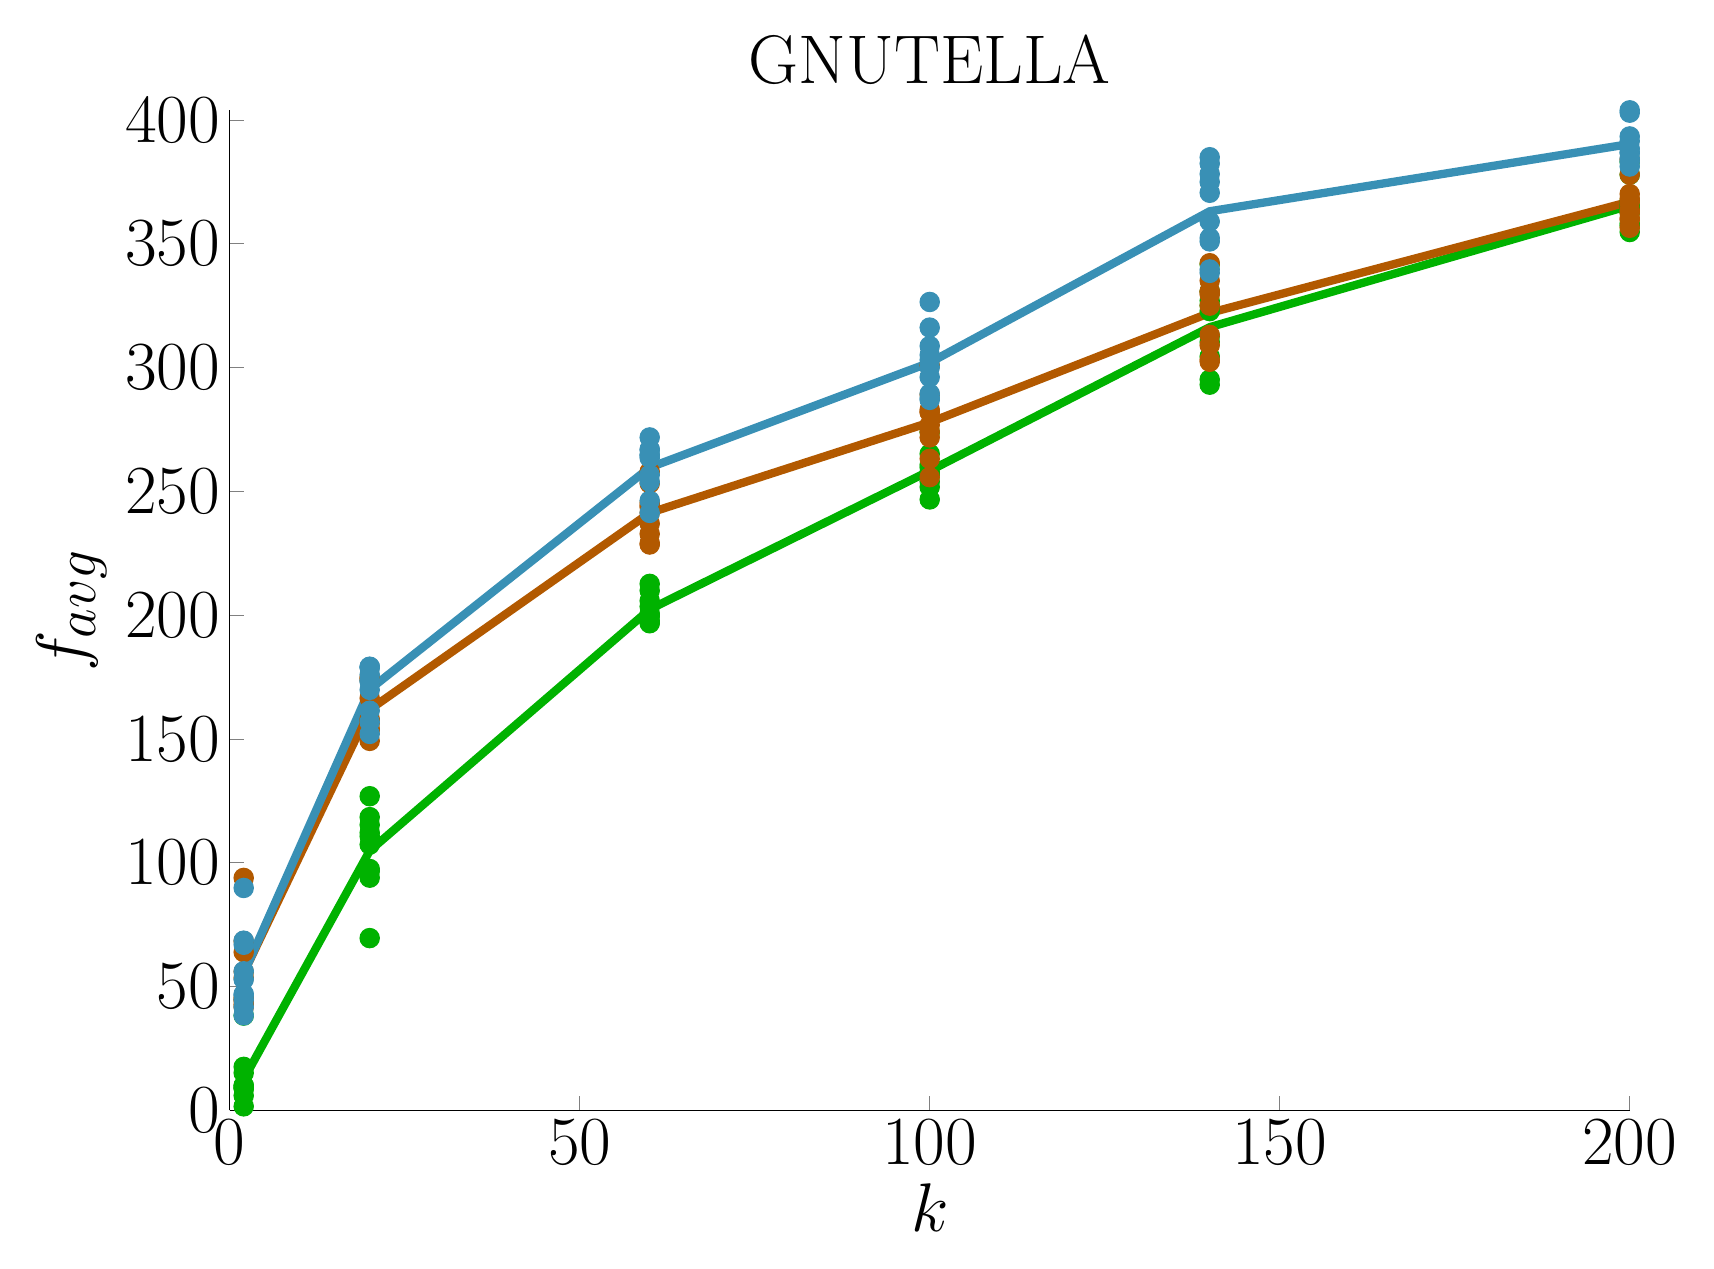
\begin{tikzpicture}

\begin{axis}[%
title style={font=\Huge},
title=GNUTELLA,
tick label style={font=\Huge},
label style={font=\Huge},
legend style={font=\Huge},
view={0}{90},
max space between ticks=50pt,
width=7in,
height=5in,
scale only axis,
xmin=0, xmax=200,
xtick={0, 50, 100, 150, 200},
xlabel={$k$},
ymin=0, ymax=403.85,
ylabel={$f_{avg}$},
major tick length=5pt,
axis lines*=left,
legend cell align=left,
clip=false]

\addplot [
only marks,
mark=*,
mark size=3.5pt,
color=green!70!black,
%solid,
%line width=2pt,
]
coordinates{
(2,1.6)(2,5.95)(2,8.8)(2,8.9)(2,9.2)(2,9.95)(2,10.0)(2,15.1)(2,17.55)(2,38.25)(20,69.55)(20,93.95)(20,96.55)(20,97.45)(20,107.3)(20,110.7)(20,112.1)(20,115.3)(20,118.4)(20,126.85)(60,196.7)(60,197.2)(60,197.55)(60,199.55)(60,199.85)(60,200.55)(60,203.4)(60,205.75)(60,209.9)(60,212.6)(100,246.7)(100,251.75)(100,253.9)(100,256.25)(100,257.25)(100,257.65)(100,259.6)(100,260.65)(100,265.1)(100,273.8)(140,293.05)(140,295.1)(140,304.4)(140,310.3)(140,312.7)(140,322.75)(140,325.1)(140,326.9)(140,330.7)(140,341.7)(200,354.7)(200,357.2)(200,358.15)(200,362.4)(200,363.15)(200,364.45)(200,365.65)(200,367.25)(200,377.85)(200,383.0)
};

\addplot [
only marks,
mark=*,
mark size=3.5pt,
color=orange!70!black,
%solid,
%line width=2pt,
]
coordinates{
(2,41.7)(2,42.8)(2,44.2)(2,44.8)(2,45.65)(2,53.5)(2,55.95)(2,63.9)(2,68.35)(2,93.85)(20,149.2)(20,153.8)(20,153.9)(20,156.45)(20,157.1)(20,158.1)(20,166.45)(20,173.7)(20,174.35)(20,175.0)(60,228.5)(60,229.0)(60,232.8)(60,236.95)(60,241.3)(60,243.6)(60,244.25)(60,245.3)(60,253.2)(60,257.95)(100,255.7)(100,263.1)(100,271.75)(100,274.1)(100,276.75)(100,281.9)(100,282.05)(100,282.95)(100,288.95)(100,300.85)(140,302.3)(140,303.15)(140,309.0)(140,313.15)(140,324.95)(140,329.45)(140,330.55)(140,330.7)(140,335.0)(140,342.1)(200,356.4)(200,359.7)(200,360.35)(200,362.6)(200,363.5)(200,366.85)(200,368.1)(200,370.05)(200,377.9)(200,384.1)
};

\addplot [
only marks,
mark=*,
mark size=3.5pt,
color=cyan!70!black,
%solid,
%line width=2pt,
]
coordinates{
(2,38.35)(2,41.75)(2,44.7)(2,46.5)(2,46.95)(2,52.85)(2,56.15)(2,66.85)(2,68.5)(2,89.8)(20,152.0)(20,156.8)(20,161.4)(20,169.8)(20,173.05)(20,173.7)(20,175.9)(20,178.85)(20,179.0)(20,179.15)(60,241.25)(60,246.2)(60,253.8)(60,256.65)(60,263.5)(60,264.4)(60,264.8)(60,266.65)(60,266.95)(60,271.75)(100,286.9)(100,287.7)(100,289.4)(100,296.1)(100,300.1)(100,303.05)(100,305.0)(100,308.65)(100,316.1)(100,326.45)(140,338.2)(140,339.6)(140,350.9)(140,352.3)(140,358.95)(140,370.55)(140,374.9)(140,378.15)(140,382.35)(140,384.9)(200,381.15)(200,383.2)(200,384.5)(200,386.65)(200,386.95)(200,388.45)(200,391.4)(200,393.3)(200,402.9)(200,403.85)
};
p
\addplot [
color=green!70!black,
solid,
line width=3pt
]
coordinates{
(2,12.53)(20,104.815)(60,202.305)(100,258.265)(140,316.27)(200,365.38)
};

\addplot [
color=orange!70!black,
solid,
line width=3pt
]
coordinates{
(2,55.47)(20,161.805)(60,241.285)(100,277.81)(140,322.035)(200,366.955)
};

\addplot [
color=cyan!70!black,
solid,
line width=3pt
]
coordinates{
(2,55.24)(20,169.965)(60,259.595)(100,301.945)(140,363.08)(200,390.235)
};


\end{axis}
\end{tikzpicture}
\end{document}
